\chapter{Implementation}
\label{ch:implementation}

\section{Introduction}

The algorithms described above were implemented in C++. For graph operations, the NetworKit and Koala libraries were used. The code is open source and available in the Koala-NetworKit GitHub repository at \url{https://github.com/krzysztof-turowski/koala-networkit/pull/46}.

All tests and benchmarks were executed on a system equipped with an AMD Ryzen 7 7800X3D 8-Core Processor and 32GB of DDR5 RAM. 

\section{Implementation details}

The repository contains separate classes for each type of problem, such as chordal graph recognition, maximum clique calculation, minimum vertex coloring, and so on. Below is a brief description of the files with their purposes:

\begin{itemize}
    \item \texttt{koala-networkit/include/recognition/ChordalGraphRecognition.hpp} \\
    The main header file defining the classes for LexBFS and MCS chordal graph recognition algorithms.
    
    \item \texttt{koala-networkit/include/coloring/ChordalVertexColoring.hpp} \\
    Header file for the class that finds the graph coloring with the minimum number of colors.
    
    \item \texttt{koala-networkit/include/clique/ChordalClique.hpp} \\
    Header file for the class that finds the maximum clique of a graph.
    
    \item \texttt{koala-networkit/include/clique\_cover/ChordalCliqueCover.hpp} \\
    Header file for the class that finds the minimum clique cover of a graph.
    
    \item \texttt{koala-networkit/include/independent\_set/ChordalIndependentSet.hpp} \\
    Header file for the class that finds the maximum independent set of a graph.
    
    \item \texttt{koala-networkit/benchmark/} \\
    Folder containing benchmarking programs to evaluate the performance of the algorithms on various graph instances.
    
    \item \texttt{koala-networkit/test/} \\
    Folder containing unit tests for checking the correctness of the implemented algorithms.
\end{itemize}

\section{Testing}

The correctness of each algorithm was tested in two ways:
\begin{enumerate}
    \item Exhaustive tests on all small-sized connected graphs, i.e., graphs with up to 10 vertices.
    \item On graphs from a benchmark suite containing random chordal and non-chordal graphs with up to $10^7$ vertices and edges.
\end{enumerate}

To generate robust and structurally varied chordal graphs in linear time, we used the subtree-intersection generator proposed by Shalom et al. (2021) \cite{Shalom2019}, available at \url{https://github.com/cmshalom/ChordalGraphGeneration}. Negative testing was performed using random Erdős–Rényi graphs to ensure the algorithms correctly reject non-chordal inputs. 

\begin{table}[H]
\centering
\begin{tabular}{llr}
\toprule
\textbf{Suite} & \textbf{Graph Topology} & \textbf{Graphs} \\
\midrule
T1: Exhaustive   & All connected $n \le 10$ & $11,989,764$ \\
T2: Medium Chordal & Shalom gen. ($n+m \sim 10^5$) & $5,000$ \\
T3: Large Chordal& Shalom gen. ($n+m \sim 10^7$) & $1,000$ \\
T4: Medium Random & Erdős-Rényi ($n=1\text{K}, m=5\text{K}$) & $10,000$ \\
T5: Large Random  & Erdős-Rényi ($n=50\text{K}, m=250\text{K}$) & $1,000$ \\
\bottomrule
\end{tabular}
\caption{Summary of correctness test suites. T1 tested all possible graphs up to $n=10$, identifying exactly $123,418$ chordal graphs \cite{OEISA048192}. T4 and T5 verified that the recognition algorithms successfully reject non-chordal structures.}
\label{tab:test_suites}
\end{table}

\section{Running time}

The algorithms were tested on several subgroups of tests. Each data point consists of the median runtime of $3$ repetitions. 

To demonstrate asymptotic scalability, the algorithms were tested across three density tiers: Sparse ($m \in O(n)$), Medium ($m \in O(n^{1.5})$), and Dense ($m \in O(n^2)$). The median runtimes, in milliseconds, are presented in Table \ref{tab:recognition_times} and Table \ref{tab:optimization_times}.

\subsection{Chordal Recognition: MCS vs. LexBFS}

Table \ref{tab:recognition_times} and Figure \ref{fig:recognition_benchmark} compare the two chordal graph recognition algorithms: Maximum Cardinality Search (MCS) and Lexicographic Breadth-First Search (LexBFS).

\begin{table}[H]
\centering
\begin{tabular}{|l|rr|rr|rr|}
\hline
& \multicolumn{2}{c|}{\textbf{Sparse}} & \multicolumn{2}{c|}{\textbf{Medium}} & \multicolumn{2}{c|}{\textbf{Dense}} \\
\hline
$n+m$ & MCS & LexBFS & MCS & LexBFS & MCS & LexBFS \\
\hline
$10^4$ & $0.238$ & $0.682$ & $0.079$ & $0.231$ & $0.036$ & $0.093$ \\
$10^5$ & $1.96$  & $5.18$  & $0.573$ & $1.38$  & $0.805$ & $2.39$  \\
$10^6$ & $14.3$  & $36.5$  & $7.79$  & $20.2$  & $6.08$  & $21.6$  \\
$10^7$ & $672$   & $1349$  & $61.7$  & $178$   & $64.0$  & $215$   \\
\hline
\end{tabular}
\caption{The running time (in ms) of the chordal recognition algorithms across density tiers.}
\label{tab:recognition_times}
\end{table}

\begin{figure}[H]
    \centering
    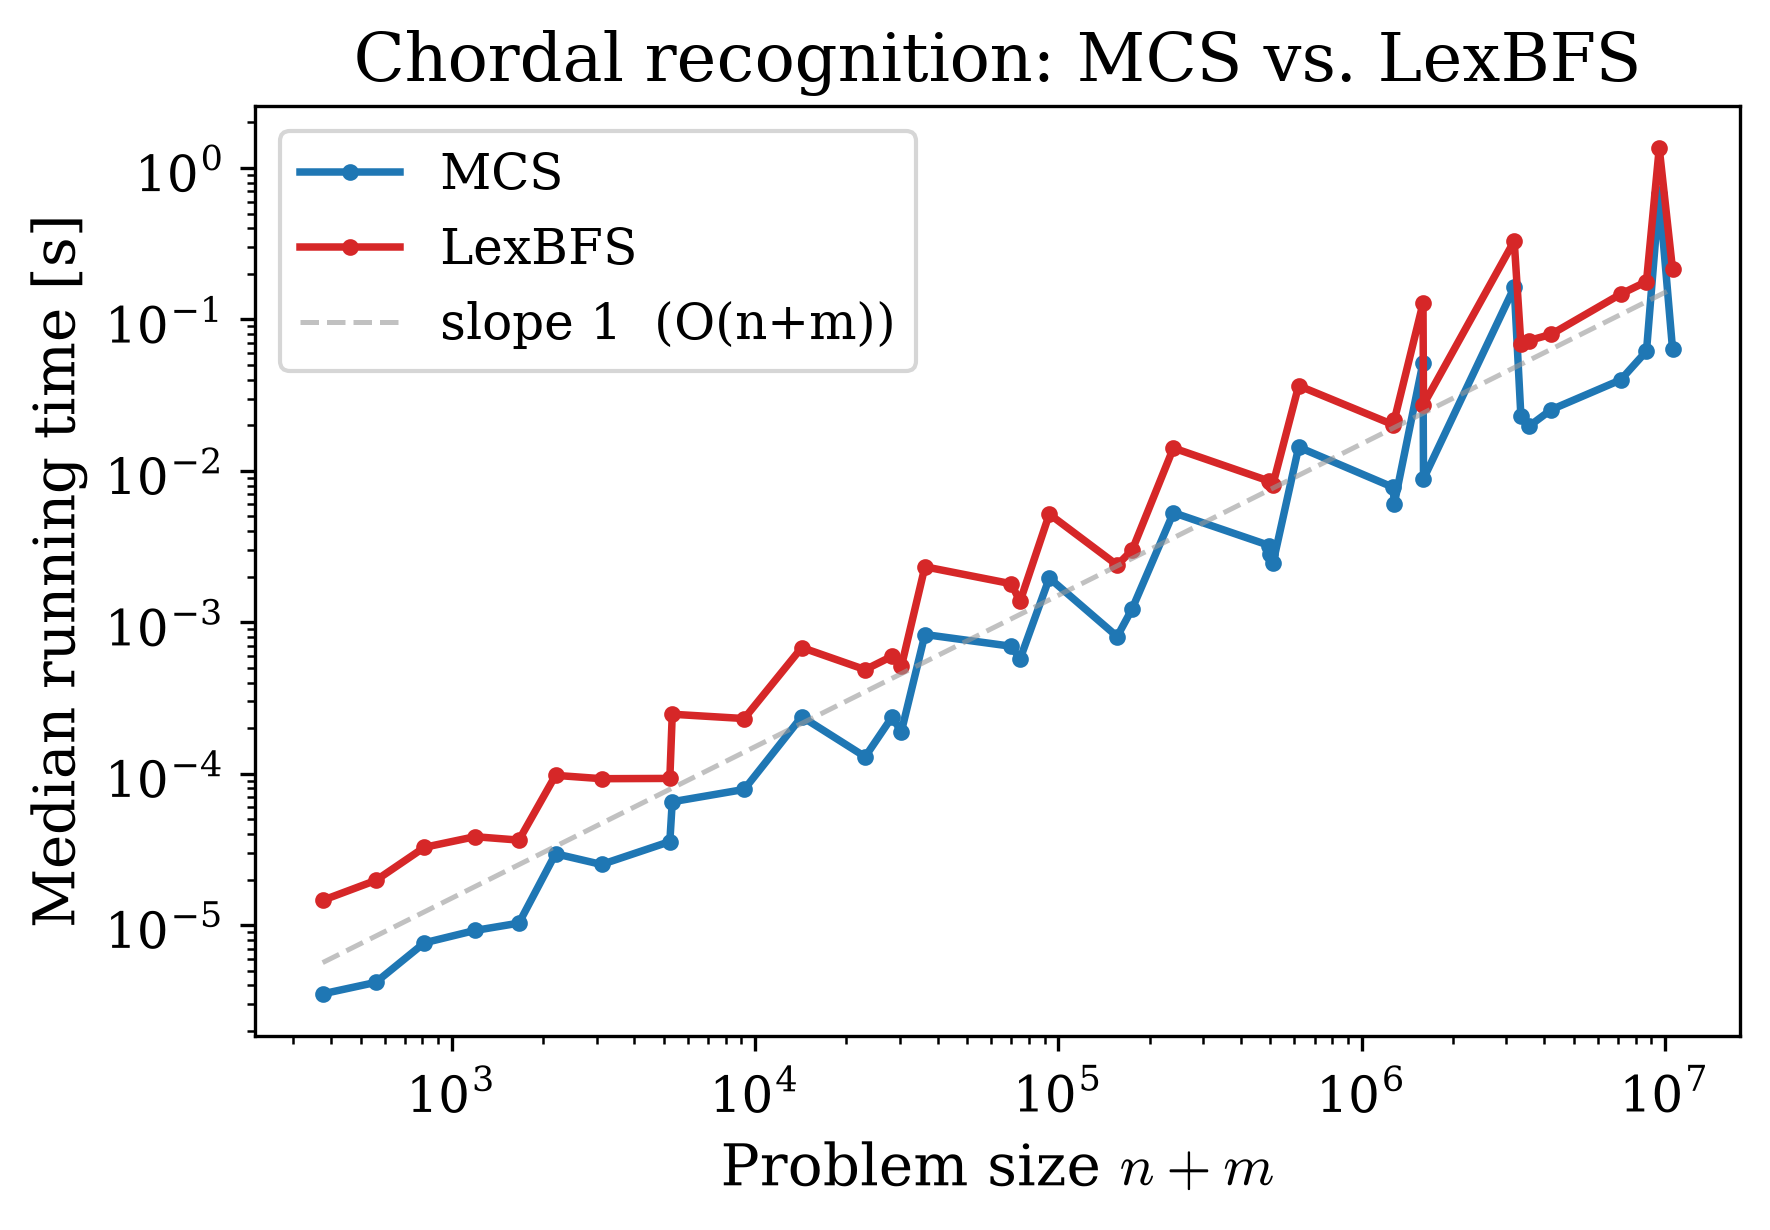
\includegraphics[width=0.75\textwidth]{images/fig_recognition.png} 
    \caption{Graph of the running time of the recognition algorithms.}
    \label{fig:recognition_benchmark}
\end{figure}

\subsection{Optimization Algorithms}

Table \ref{tab:optimization_times} shows the running times of the four PEO-based optimization algorithms. The time required to compute the PEO is excluded. The scaling behaviors across the sparse, medium, and dense density tiers are plotted sequentially in Figure \ref{fig:optimization_sparse}, Figure \ref{fig:optimization_medium}, and Figure \ref{fig:optimization_dense}.

\begin{table}[H]
\centering
\begin{tabular}{lrrrr}
\toprule
\boldmath$n+m$ & \textbf{Coloring} & \textbf{Max Clique} & \textbf{Clique Cover} & \textbf{Ind. Set} \\
\midrule
\multicolumn{5}{l}{\textbf{Medium} ($m \in O(n^{1.5})$)} \\
\midrule
$10^4$         & $0.036$  & $0.010$ & $0.011$ & $0.002$ \\
$10^5$         & $0.198$  & $0.081$ & $0.034$ & $0.011$ \\
$10^6$         & $2.52$   & $1.27$  & $0.255$ & $0.101$ \\
$10^7$         & $28.1$   & $17.9$  & $1.13$  & $0.576$ \\
\midrule
\multicolumn{5}{l}{\textbf{Dense} ($m \in O(n^2)$)} \\
\midrule
$10^4$         & $0.013$  & $0.004$ & $0.002$ & $0.001$ \\
$10^5$         & $0.265$  & $0.120$ & $0.006$ & $0.002$ \\
$10^6$         & $1.86$   & $0.870$ & $0.019$ & $0.005$ \\
$10^7$         & $20.9$   & $13.7$  & $0.083$ & $0.033$ \\
\bottomrule
\end{tabular}
\caption{The running time (in ms) of the optimization algorithms across the medium and dense density tiers.}
\label{tab:optimization_times}
\end{table}

\begin{figure}[H]
    \centering
    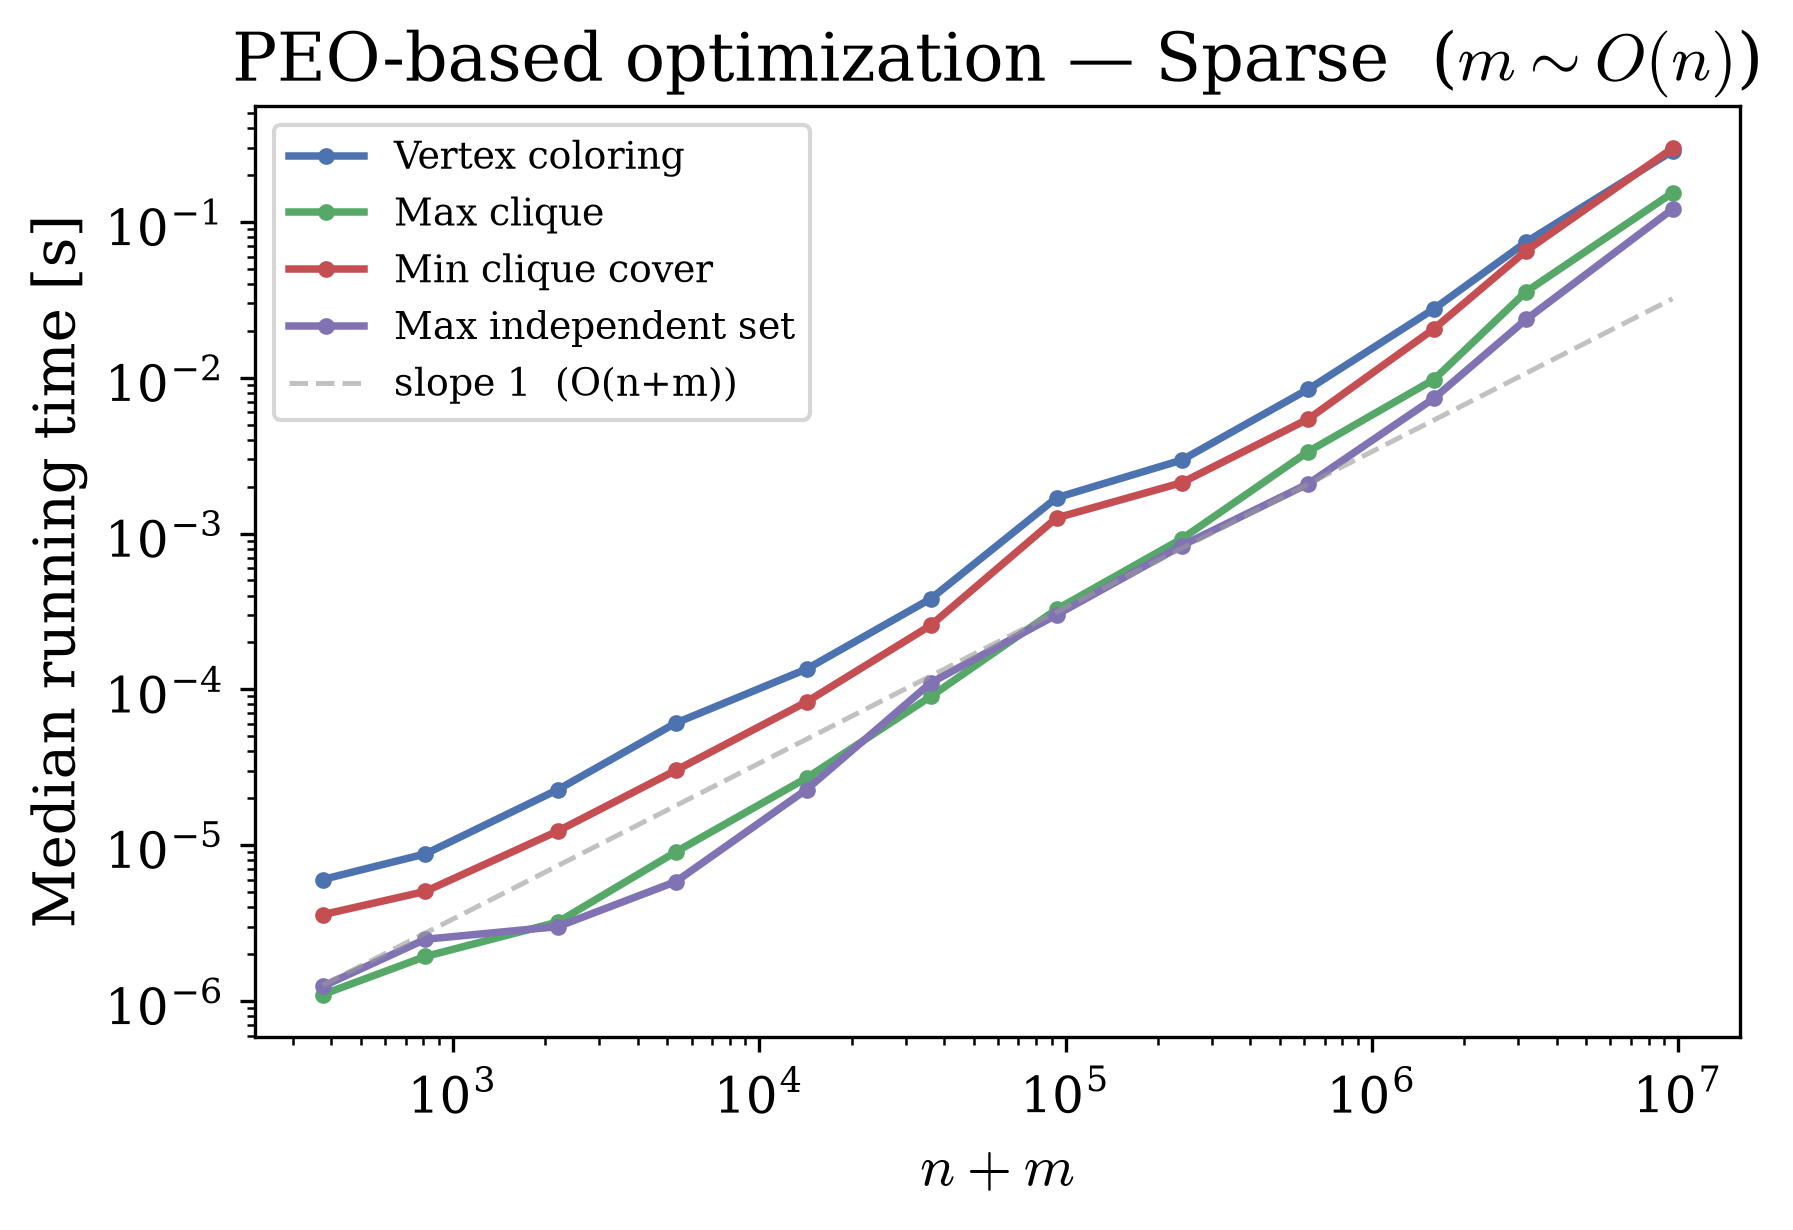
\includegraphics[width=0.75\textwidth]{images/fig_optimization_sparse.png}
    \caption{Graph of the running time of the optimization algorithms on the sparse density tier.}
    \label{fig:optimization_sparse}
\end{figure}

\begin{figure}[H]
    \centering
    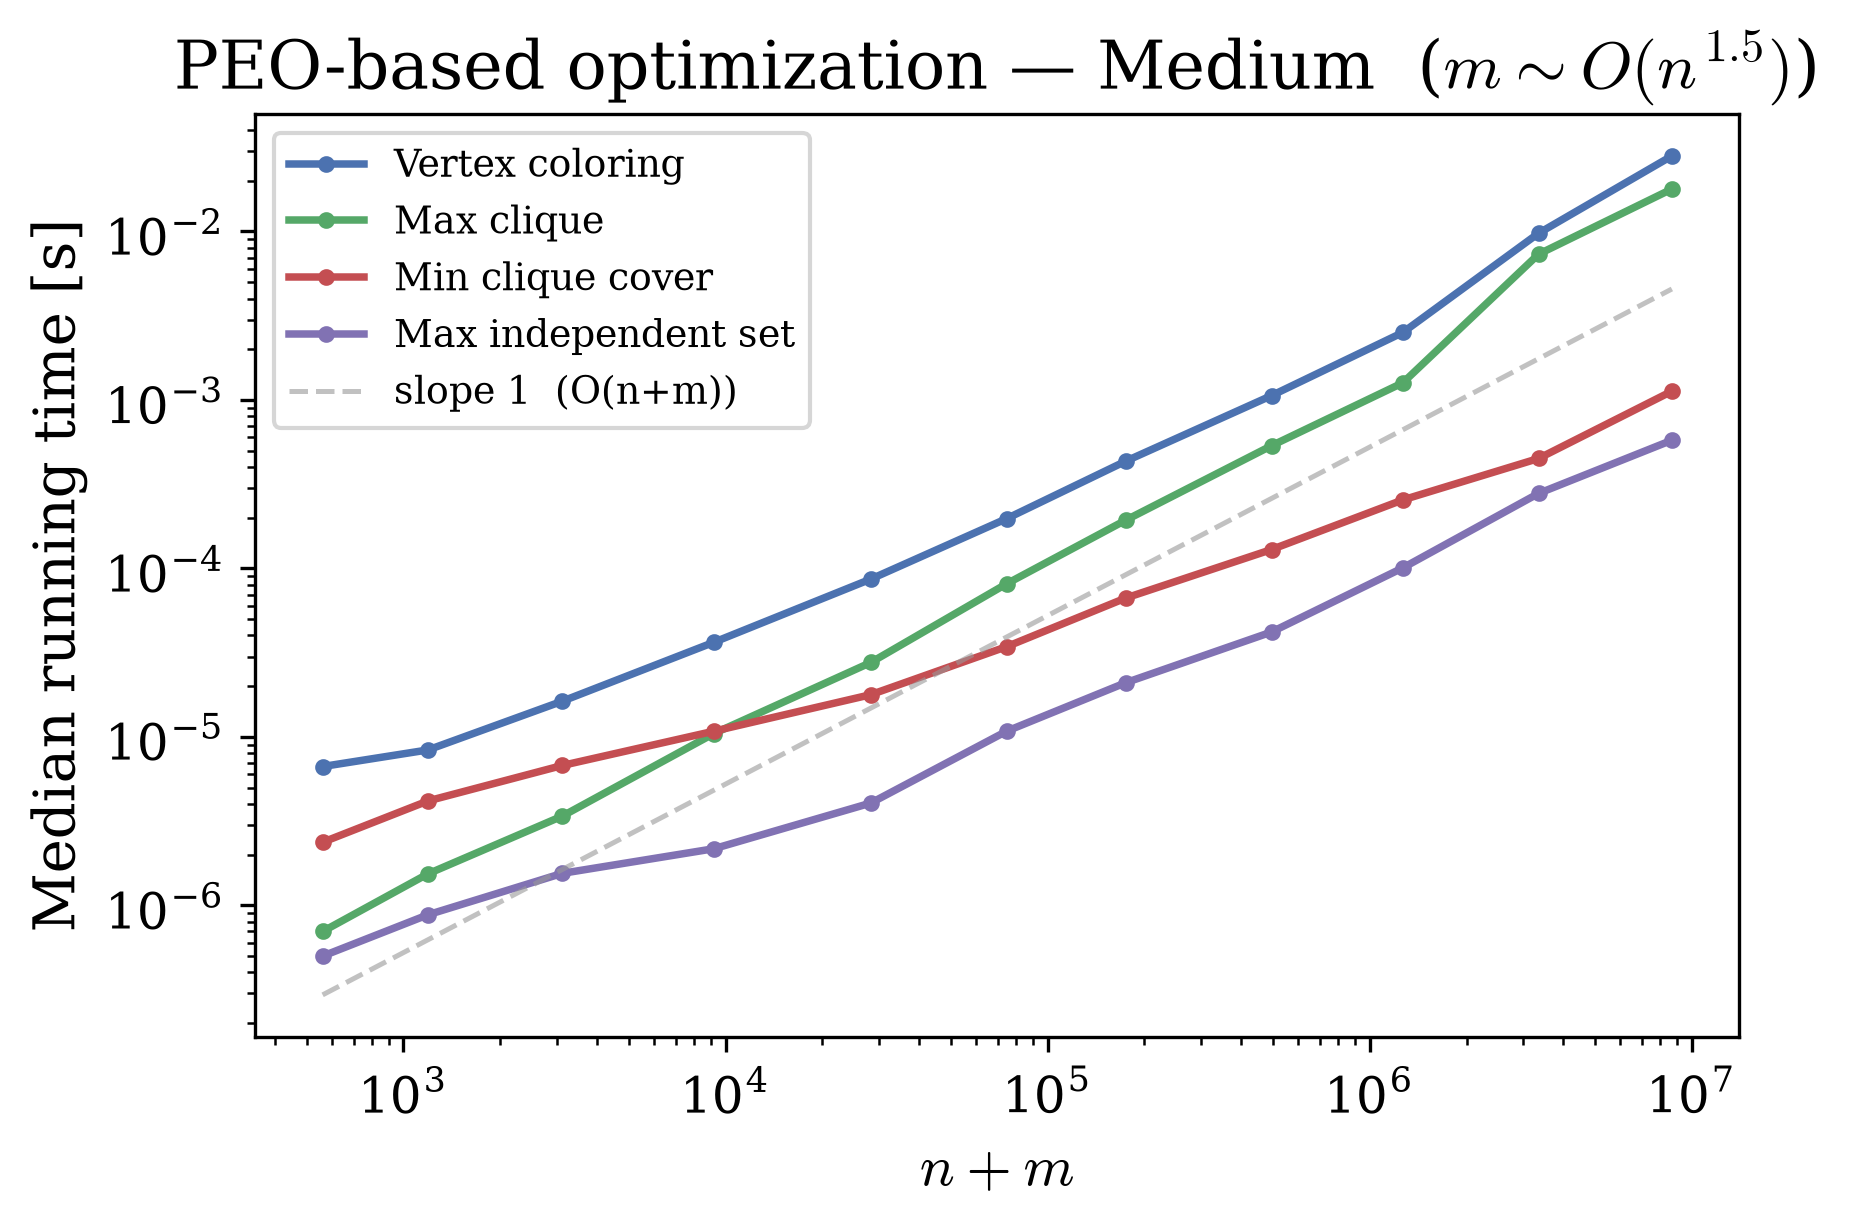
\includegraphics[width=0.75\textwidth]{images/fig_optimization_medium.png}
    \caption{Graph of the running time of the optimization algorithms on the medium density tier.}
    \label{fig:optimization_medium}
\end{figure}

\begin{figure}[H]
    \centering
    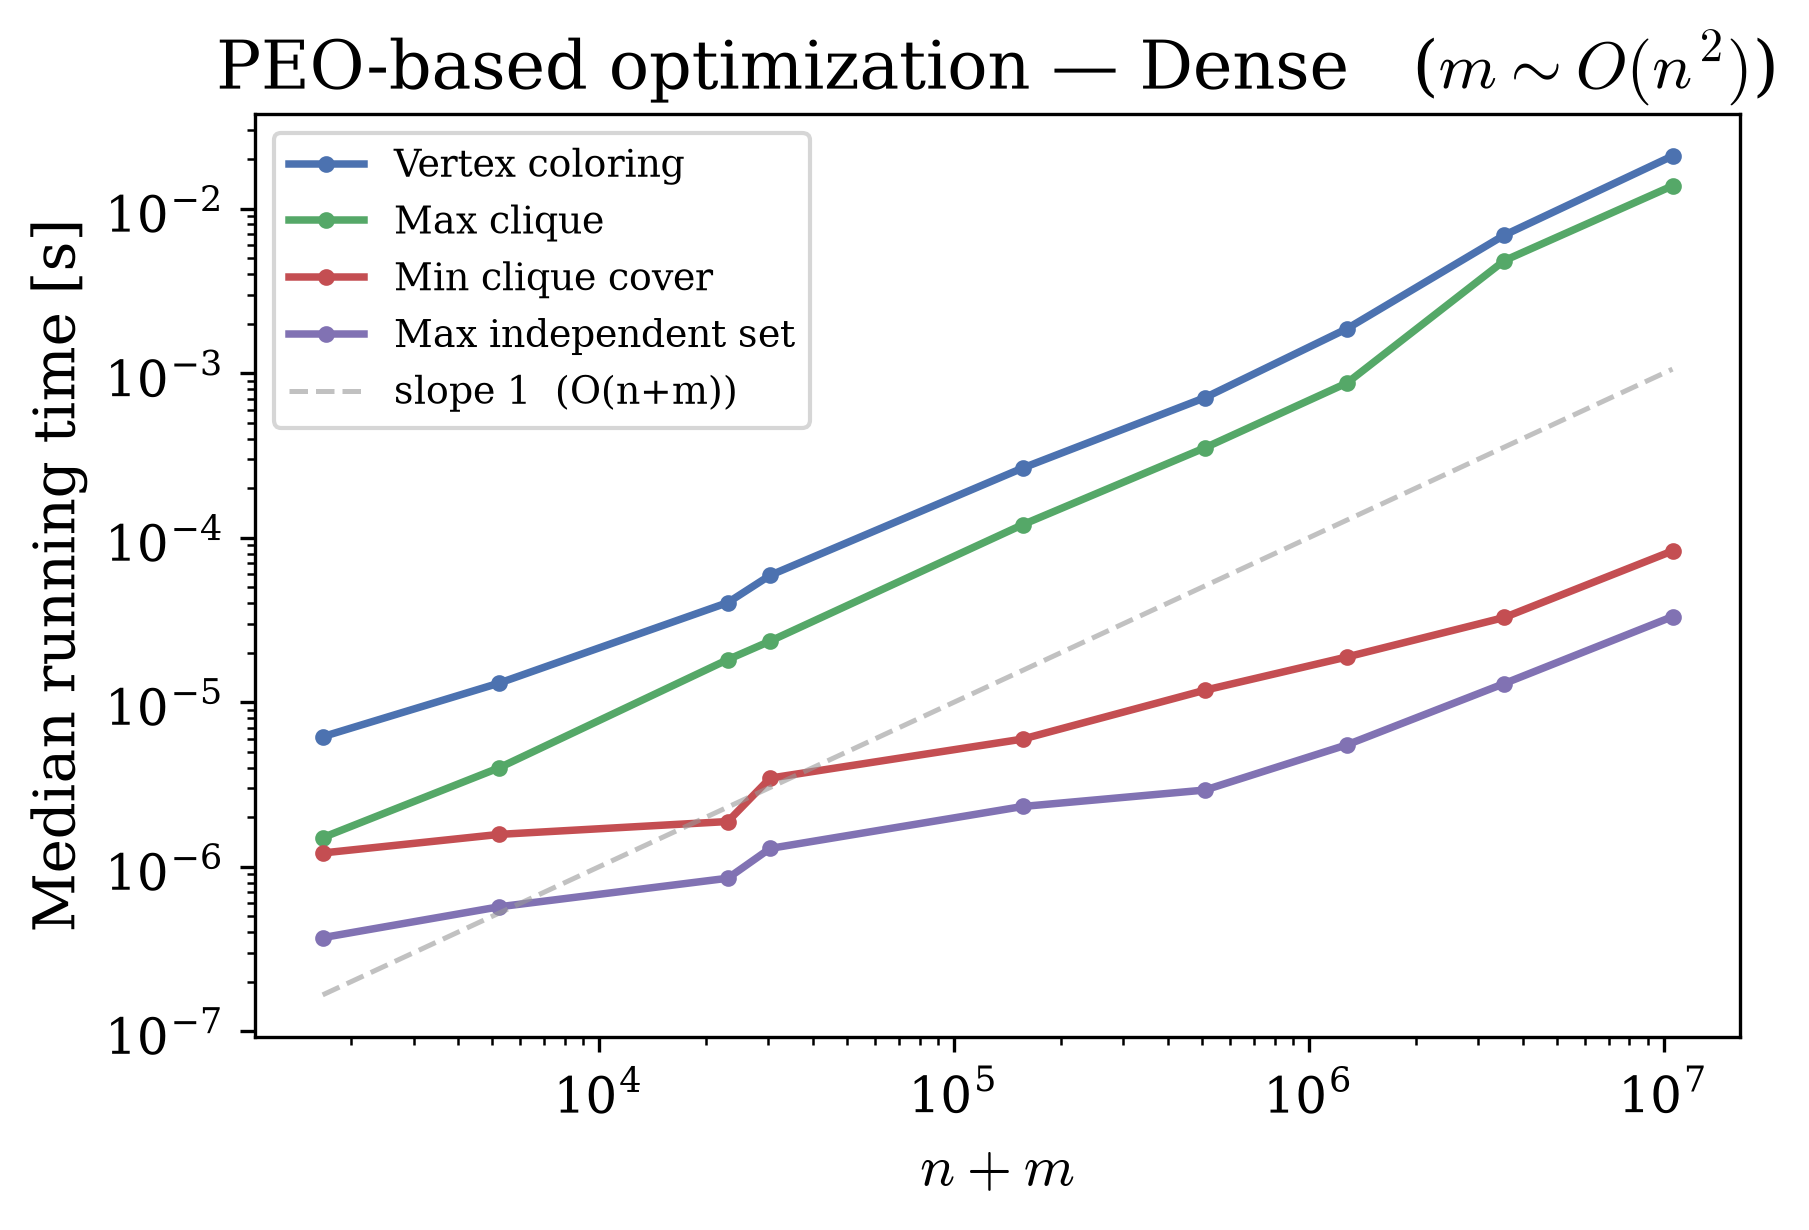
\includegraphics[width=0.75\textwidth]{images/fig_optimization_dense.png}
    \caption{Graph of the running time of the optimization algorithms on the dense density tier.}
    \label{fig:optimization_dense}
\end{figure}

\subsection{The Impact of Density}

To isolate the impact of the number of edges, an additional benchmark was performed with a fixed vertex count of $n = 5000$, scaling the edge density from $0.5\%$ to $90\%$. The results are shown in Table \ref{tab:density_impact} and Figure \ref{fig:density_impact}.


\begin{table}[H]
\centering
\begin{tabular}{|l|r|rrrrrr|}
\hline
\textbf{Density} & \textbf{Edges ($m$)} & \textbf{A1} & \textbf{A2} & \textbf{A3} & \textbf{A4} & \textbf{A5} & \textbf{A6} \\
\hline
$0.005$  & $64{,}831$      & $0.684$ & $1.855$  & $0.308$  & $0.098$ & $0.088$ & $0.023$ \\
$0.040$  & $494{,}797$     & $2.87$  & $8.14$   & $0.895$  & $0.417$ & $0.058$ & $0.015$ \\
$0.150$  & $1{,}592{,}650$ & $8.68$  & $26.1$   & $3.30$   & $1.26$  & $0.051$ & $0.019$ \\
$0.450$  & $4{,}207{,}022$ & $24.1$  & $79.4$   & $8.59$   & $4.30$  & $0.042$ & $0.021$ \\
$0.900$  & $7{,}132{,}201$ & $36.0$  & $138$    & $13.0$   & $8.13$  & $0.042$ & $0.014$ \\
\hline
\end{tabular}
\caption{The running time (in ms) showing the density impact for a fixed \\$n=5000$. The identifiers denote the following algorithms: A1 (MCS Recognition), A2 (LexBFS Recognition), A3 (Vertex Coloring), A4 (Maximum Clique), A5 (Minimum Clique Cover), and A6 (Maximum Independent Set).}
\label{tab:density_impact}
\end{table}

\begin{figure}[H]
    \centering
    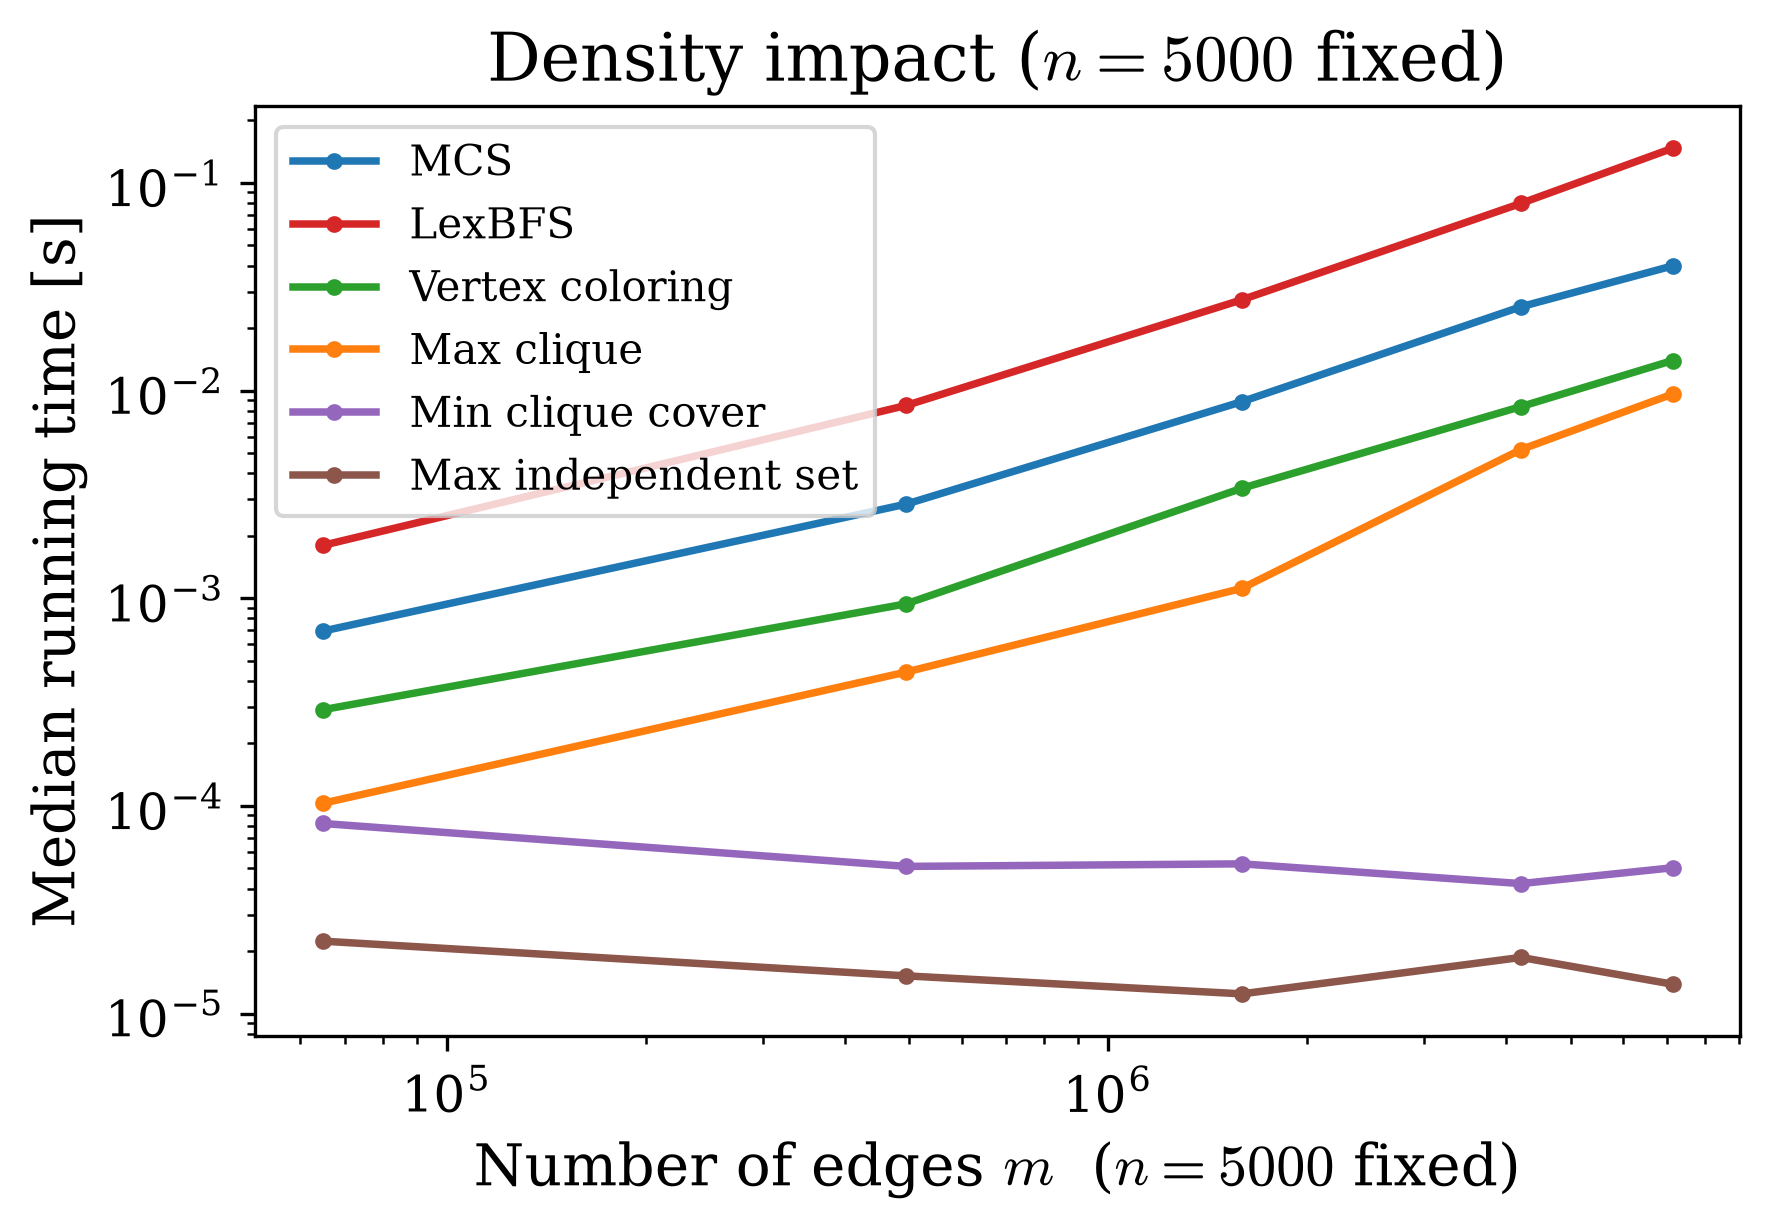
\includegraphics[width=0.75\textwidth]{images/fig_density_impact.png}
    \caption{Graph of the running time showing density impact for fixed \\$n=5000$.}
    \label{fig:density_impact}
\end{figure}


\subsection{Constant Factor Analysis}

An ordinary least-squares linear regression was performed to estimate the constant factor $\alpha$ (in nanoseconds per unit of $n+m$) representing the processing overhead of each algorithm. Across all density tiers, the recognition algorithms exhibit the largest constant overheads, with MCS consistently demonstrating lower overhead than LexBFS. The sparse-tier constants are elevated compared to medium and dense, reflecting cache effects: sparse graphs at large scale have many vertices with small degrees, causing frequent cache misses in the recognition data structures. The optimization algorithms show much smaller constants. Notably, the constant factors for clique cover and independent set drop by multiple orders of magnitude in denser graphs, empirically confirming that these greedy algorithms bypass redundant operations as the search space structurally shrinks.


\begin{table}[h!]
\centering
\small
\begin{tabular}{|l|c|c|c|c|}
\hline
\textbf{Algorithm} & \textbf{All Tiers $\alpha$} & \textbf{Sparse $\alpha$} & \textbf{Medium $\alpha$} & \textbf{Dense $\alpha$} \\
\hline
MCS & $26.91$ & $69.15$ & $7.087$ & $6.040$ \\
LexBFS & $59.04$ & $138.84$ & $20.49$ & $20.36$ \\
Coloring & $11.26$ & $29.45$ & $3.210$ & $1.978$ \\
Max Clique & $6.245$ & $15.79$ & $2.080$ & $1.313$ \\
Min Clique Cover & $9.961$ & $30.41$ & $0.1277$ & $0.00756$ \\
Max Independent Set & $4.042$ & $12.32$ & $0.0676$ & $0.00305$ \\
\hline
\end{tabular}
\caption{Estimated constant factor $\alpha$ (in nanoseconds per unit of $n+m$) for the linear regression model $\text{Time} = \alpha(n+m)$ across individual and combined density tiers.}
\label{tab:ols_complexity_analysis}
\end{table}



\section{Conclusions}

The running time of the algorithms depends on both the number of edges and the number of vertices. From the figures and tables, it is clear that the algorithms are linear within the tested range, confirming the $O(n+m)$ theoretical complexity. 

The analysis of the constant factor $\alpha$ reveals that MCS has lower constant overhead than LexBFS, making it the faster choice for recognition in practice. For the optimization algorithms, while coloring and clique scale directly with the graph size, the clique cover and independent set algorithms benefit from the structural properties of dense graphs, which significantly reduces their execution overhead.


